\documentclass[10pt]{article}
\usepackage{icmlko}

\icmlmeta{IP 파운데이션 월드모델}{281}{손잡이 하나}{노트 276이 예측하고 280이 ``확인''한 40행 계단이 없다 --- 계단은 20 바로 위에 있고, 점이 없어서 두 배로 읽었다}

\begin{document}

\twocolumn[
\icmlheader

\begin{abstract}
노트 280의 청력 곡선은 도메인 다섯을 가로질렀다 --- 그래서 \textbf{행 수}와
\textbf{어느 도메인인가}가 붙어 있었다. 웹툰 하나만 놓고 \textbf{학습 라벨을
지워} 행을 줄였다(유보는 안 건드린다). 두 가지가 나왔다. \textbf{하나 ---
교락은 없다.} 웹툰을 16행으로 줄이면 F6 $+$0.5370 · F18 $+$0.0000 · F10
$+$0.0000 인데, 노트 280의 \emph{팝업} 16행이 $+$0.5272 · $+$0.0000 ·
$+$0.0000 이었다. 거의 같다. \textbf{둘 --- 그런데 계단이 40에 없다.}
노트 276이 ``양쪽 잎을 채우려면 $2{\times}20{=}40$''이라 쓰고 노트 280이
``예측한 자리에 있다''고 확인했는데, 30행에서 이미 $+$0.1419 다. 16$\sim$40을
촘촘히 훑으니 \textbf{20까지 정확히 0, 22에서 $+$0.0765} 다. \textbf{문턱은
잎 하한 그 자체지 두 배가 아니다} --- 특수 열의 반대쪽 잎에는 언제나 채움값
0.5 인 수천 행이 있으니 채워야 할 잎은 하나뿐이다. 노트 280이 확인했다고
믿은 까닭은 \textbf{팝업 16과 아이돌 54 사이에 점이 없어서} 20과 40을 못
갈랐기 때문이다. \textbf{맞는 예측을 틀린 이유로 확인했다.} 덤으로 F10의
문턱도 잡혔다 --- 200행까지 0 이다가 400행에서 $+$0.7354 이고, 그 값이
2,106행과 \emph{소수 넷째 자리까지 같다}. 배합 선택이 이산이라는 뜻이다.
그리고 이 실험이 \texttt{guards.\_split} 에 남아 있던 노트 273의 병
(``어느 행이 진짜 있는 행인가'')을 \textbf{다섯 번째}로 드러냈다 ---
\texttt{rank.predictions} 가 그 함수를 쓰므로 이 세션의 짝 측정이 전부 그
경로를 지났다(지금 판에서는 no-op 확인).
\end{abstract}
]

\section{두 점 사이에 점이 없었다}

노트 280이 곡선을 그렸다 --- 팝업 16 · 아이돌 54 · 도서 80 · 게임 259 ·
웹툰 2,106. 나무(F8 · F18)가 16에서 0 이고 54에서 $+$0.57$\sim$0.66 이었다.
노트 276이 \texttt{min\_samples\_leaf}$=$20 에서 ``$2{\times}20{=}40$''을
예측해 놨으니 \textbf{계단이 예측한 자리에 있다}고 적었다.

\textbf{16과 54 사이에는 점이 하나도 없다.} 20이든 40이든 그 자료로는 똑같이
보인다. 그리고 그 곡선은 도메인을 가로질렀으므로 행 수가 원인인지 도메인이
원인인지도 안 갈린다(게임 259가 전체적으로 눌려 있던 것이 그 신호였다).

그래서 \textbf{웹툰 하나}만 쓰고 학습 라벨을 무작위로 지워 행을 줄였다.
유보는 2025년 이후라 안 건드린다.

\section{교락은 없다}

\begin{figure*}[t]
\centering
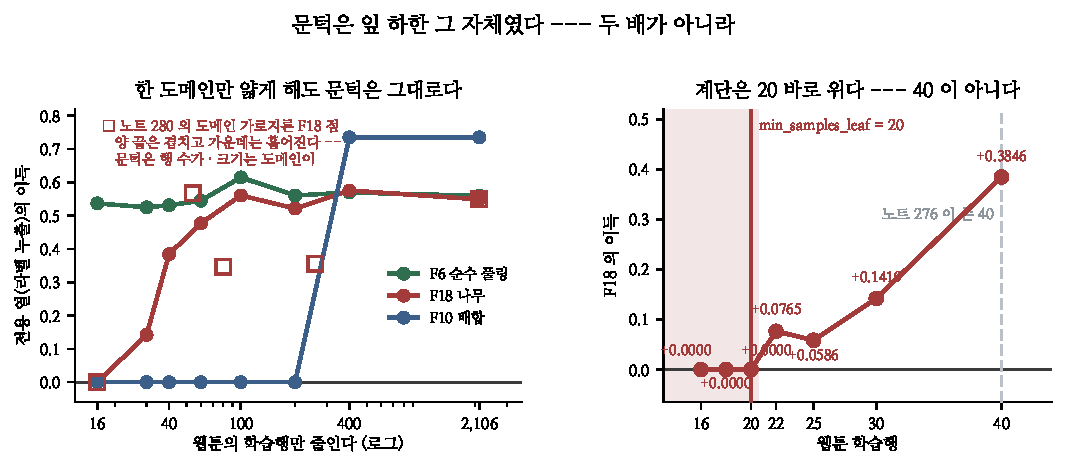
\includegraphics[width=\textwidth]{figs/knob.pdf}
\caption{왼쪽 --- 웹툰의 학습행만 줄인 곡선. 빈 사각형이 노트 280의 도메인
가로지른 F18 점이다. 오른쪽 --- 16$\sim$40 을 촘촘히 훑은 것. 붉은 선이
\texttt{min\_samples\_leaf}$=$20, 회색 점선이 노트 276이 쓴 40.}
\end{figure*}

\begin{center}\small
\begin{tabular}{lrrr}
\hline
웹툰 학습행 & F6 & F18 & F10 \\
\hline
16 & $+$0.5370 & \textbf{$+$0.0000} & $+$0.0000 \\
30 & $+$0.5252 & $+$0.1419 & $+$0.0000 \\
40 & $+$0.5313 & $+$0.3846 & $+$0.0000 \\
60 & $+$0.5451 & $+$0.4769 & $+$0.0000 \\
100 & $+$0.6150 & $+$0.5608 & $+$0.0000 \\
200 & $+$0.5607 & $+$0.5216 & $+$0.0000 \\
400 & $+$0.5697 & $+$0.5757 & \textbf{$+$0.7354} \\
2,106 & $+$0.5597 & $+$0.5490 & \textbf{$+$0.7354} \\
\hline
\end{tabular}
\end{center}

웹툰 16행: F6 $+$0.5370 · F18 $+$0.0000 · F10 $+$0.0000.
노트 280의 \emph{팝업} 16행: $+$0.5272 · $+$0.0000 · $+$0.0000.
\textbf{다른 도메인인데 거의 같다.} 문턱을 정하는 것은 행 수다.

\paragraph{다만 크기는 도메인이 정한다} 그림의 빈 사각형(노트 280의 도메인
가로지른 점)은 \textbf{양 끝에서만 겹치고 가운데는 흩어진다} --- 아이돌 54는
곡선보다 위, 도서 80과 게임 259는 아래다. \textbf{문턱은 행 수가 정하고
문턱 위의 크기는 도메인이 정한다}(게임은 정상 $\rho$ 가 이미 0.62라 올릴
자리가 좁다). 노트 280의 곡선을 ``청력 곡선''이라 부른 것은 문턱에 대해서만
맞다.

\section{그런데 계단이 40에 없다}

30행에서 이미 $+$0.1419 다. 40이 문턱이면 0 이어야 한다. 16$\sim$40을 촘촘히
훑었다.

\begin{center}\small
\begin{tabular}{rrrr}
\hline
웹툰 학습행 & 정상 & 누출 & 이득 \\
\hline
16 & 0.2264 & 0.2264 & $+$0.0000 \\
18 & 0.2531 & 0.2531 & $+$0.0000 \\
\textbf{20} & 0.2502 & 0.2502 & \textbf{$+$0.0000} \\
\textbf{22} & 0.2333 & 0.3098 & \textbf{$+$0.0765} \\
25 & 0.2688 & 0.3274 & $+$0.0586 \\
30 & 0.2870 & 0.4290 & $+$0.1419 \\
40 & 0.2751 & 0.6597 & $+$0.3846 \\
\hline
\end{tabular}
\end{center}

\textbf{20까지 정확히 0, 22에서 살아난다.} 계단은 \texttt{min\_samples\_leaf}
그 자체에 있다.

\paragraph{왜 두 배가 아닌가} 노트 276의 추론은 ``양쪽 잎을 다 채워야 하니
$2{\times}20$''이었다. \textbf{틀렸다.} 이 열은 그 도메인 행에서만 값이
변하고 나머지 8,000여 행은 전부 채움값 0.5 다. 그러니 특수 행을 한쪽으로
가르면 \textbf{반대쪽 잎에는 언제나 수천 행이 있다.} 채워야 할 잎은
하나뿐이고, 그 하나에 20이 필요하다.

20이 아니라 22에서 넘는 것도 설명이 된다 --- F18은 부트스트랩 배깅이라
각 자루가 특수 행을 평균만큼만 가진다. 정확히 20이면 자루 대부분이 20을
못 채운다.

\paragraph{맞는 예측을 틀린 이유로 확인했다} 이게 이 노트의 요점이다.
노트 276이 ``40''을 예측했고, 노트 280이 ``16에서 0, 54에서 큼''을 보고
\textbf{확인됐다}고 적었다. 그 자료는 20과 40을 못 가른다. \textbf{예측이
맞았다고 느낀 것은 점이 없었기 때문이다.} 노트 187의 값싼 검사가 ``안
움직이면 안 닿은 것''이었다면 여기서는 그 짝이 필요하다 --- \textbf{맞았다고
느껴지면 그 사이에 점이 있는지 본다.}

\section{덤 둘}

\paragraph{F10의 문턱} 200행까지 0 이다가 400행에서 $+$0.7354 이고, 2,106행에서도
\textbf{$+$0.7354로 똑같다}(소수 넷째 자리까지). 도메인별 배합 선택이
\textbf{이산}이라는 뜻이다 --- 한번 ``제 이력'' 쪽으로 넘어가면 전용 열이
최대로 일하고, 그 뒤로는 행을 다섯 배 늘려도 안 변한다. F10의 문턱은 나무의
20보다 \textbf{열 배 이상} 높다.

\paragraph{같은 병의 다섯 번째 자리} 이 실험이 학습 라벨을 일부러 지우자
\texttt{guards.\_split} 이 \texttt{Input y contains NaN} 으로 죽었다. 노트
273이 \texttt{harness.evaluate} 에서 고친 바로 그것이 여기 남아 있었다 ---
연도로만 자르고 라벨 유한을 안 본다. \textbf{\texttt{rank.predictions} 가
이 함수를 쓴다} --- 이 세션의 짝 측정이 전부 이 경로를 지났다. 지금 판은
2025년 이전 결측이 0건이라 두 마스크가 같아서 안 물렸고, 고친 뒤 판 0.4845 ·
팝업 0.3614 · 웹툰 0.4533 이 넷째 자리까지 불변임을 확인했다. \textbf{노트
271이 셋, 273이 넷째, 이번이 다섯째다.}

\paragraph{고칠 것} \texttt{lab/hearing.py} 가 나무 계열 문턱을
\texttt{2 * min\_samples\_leaf} 로 적고 있다. \textbf{\texttt{min\_samples\_leaf}
로 고친다}(안전 여유로 $+$2). 이 노트와 함께 고쳤다.

\paragraph{남은 것}
\begin{center}\small
\begin{tabular}{ll}
\hline
갈래 & 왜 \\
\hline
F10 문턱 좁히기 & 200$\sim$400 사이. 이산 전환점 \\
잎 하한을 손잡이로 & 5로 내리면 팝업이 산다(노트 276) \\
진짜 축으로 & 이 곡선은 전부 라벨 누출 --- 상한이다 \\
아이돌 학습행 & 2호 도메인 설계에 이 수가 필요하다 \\
\hline
\end{tabular}
\end{center}

\paragraph{규약} \textbf{예측이 맞았다고 느껴지면 그 사이에 점이 있는지
본다.} 노트 280은 두 점으로 계단 위치를 ``확인''했는데 그 두 점이 20과 40을
못 갈랐다. 반증만 통제가 필요한 게 아니라 \textbf{확인도 통제가 필요하다} ---
이 세션에서 내 주장이 좁혀진 네 번째이고(277 · 278 · 279 · 281), 앞의 셋은
반증이었지만 이번 것은 \textbf{맞은 결론의 틀린 근거}였다.

\end{document}
